\documentclass[12pt]{beamer}

\usepackage{amsmath}
\usepackage{amssymb}
\usepackage{graphics, subfigure}
%\pagestyle{empty}
% \usepackage{slashbox}
\usepackage{colortbl}
\usepackage{color}
\usepackage{blindtext}
\usepackage{scrextend}
\newcommand{\hilight}[1]{\colorbox{yellow}{#1}}
%\usepackage{soul}

\usepackage{graphicx}
\usetheme[secheader]{Madrid}
\usefonttheme[stillsansserifsmall]{serif}
\usefonttheme[onlylarge]{structurebold}
\usecolortheme[RGB={10,120,100}]{structure}
\setbeamertemplate{navigation symbols}{}

%\input{defs}


% \titlegraphic{\includegraphics[width=22mm]{figures/Kinv}}

% \begin{figure}[h!]
%     % \begin{center}
%     \centering
%     \includegraphics[width=80mm]{figures/Eigen}
%     % \end{center}
%     \caption{Real part of eigenvalues of preconditioned matrix $\re{\mathcal{P}_{\rm schurMH}^{-1} \mathcal{K}_{\rm MH}}$ (imaginary parts small)}
% \end{figure}

% \institute[]{University of British Columbia}

\definecolor{darkgreen}{rgb}{0,0.5,0}
\definecolor{darkyellow}{rgb}{.8,.6,.04}
\newcommand{\gr}[1]{\textcolor{darkgreen} {#1}}
\newcommand{\wh}[1]{\textcolor{white}     {#1}}
\newcommand{\dy}[1]{\textcolor{darkyellow}{#1}}
\newcommand{\yb}[1]{\colorbox {yellow}    {#1}}
\newcommand{\re}[1]{{\textcolor{red}       {#1}}}
\newcommand{\bl}[1]{{\textcolor{blue}{#1}}}
\newcommand{\w}[1]{{\textcolor{white}{#1}}}

\newcommand{\RE}[1]{{\bf\textcolor{red}       {#1}}}
\newcommand{\GR}[1]{{\bf\textcolor{darkgreen} {#1}}}
\newcommand{\DY}[1]{{\bf\textcolor{darkyellow}{#1}}}
\newcommand{\BL}[1]{{\bf\textcolor{blue}{#1}}}
\newcommand{\ssec}[1]{{\bf #1}}
\newcommand{\rsec}[1]{{\bf\color{red}       #1}}
\newcommand{\bsec}[1]{{\bf\color{blue}      #1}}
\newcommand{\gsec}[1]{{\bf\color{darkgreen} #1}}
\newcommand{\dom}{\mbox{\sf dom}}

\newcommand{\curl}{\ensuremath{\nabla\times\,}}
\renewcommand{\div}{\nabla\cdot\,}
\newcommand{\grad}{\ensuremath{\nabla}}

\usepackage[utf8]{inputenc}
\usepackage{array}


\newcommand{\R}{\mathbb{R}}
\newcommand{\minim}{\mathop{\mathrm{minimize}}}
\newcommand{\minimize}[1]{\displaystyle\minim_{#1}}
\newcommand{\maxim}{\mathop{\mathrm{maximize}}}
\newcommand{\maximize}[1]{\displaystyle\maxim_{#1}}
\newcommand{\st}{\mathop{\mathrm{subject\ to}}}
\newcommand{\Null}{\mathop{\mathrm{Null}}}
\newcommand{\A}{\mathcal{A}}
\newcommand{\I}{\mathcal{I}}
\newcommand{\kns}{\mathcal{K}_{\rm NS}}
\newcommand{\km}{\mathcal{K}_{\rm M}}
\newcommand{\kc}{\mathcal{K}_{\rm C}}

\newcommand{\aheader}[2]{\action{#2}}
% first argument: slide number to appear from, second argument: content of header
\newcommand{\hiddencell}[2]{\action<#1->{#2}}
% first argument: slide number to appear from, second argument: content of cell


\title{Algebraic Multigrid}
\author{Michael Wathen}
\institute{UBC Computer Science}
\date{8$^{\tiny{\mbox{th}}}$ April 2016}

\begin{document}

\begin{frame}

\title{Algebraic Multigrid}
\titlepage
\title{Algebraic Multigrid}

\end{frame}

\title{Algebraic Multigrid}
% \section{Introduction}

% \begin{frame}

% \frametitle{Continuous and Discrete Maxwell's equations}
% \begin{tabular}{lrrrr}
% \hline
% {} &  Grid size &      DoF &  $\#$ iters &  Soln Time \\
% \hline
% 0 &       $   2^3$ &       81 &        1 &   4.25e-04 \\
% 1 &       $   4^3$ &      375 &        3 &   6.03e-04 \\
% 2 &       $   8^3$ &     2187 &        5 &   2.53e-03 \\
% 3 &      $  16^3$ &    14739 &        5 &   1.96e-02 \\
% 4 &      $  32^3$ &   107811 &        6 &   2.24e-01 \\
% 5 &      $  64^3$ &   823875 &        6 &   2.28e+00 \\
% 6 &     $ 128^3$ &  6440067 &        6 &   2.09e+01 \\
% \hline
% \end{tabular}

% \end{frame}

\section{Problem}
\begin{frame}{Problem?}
\begin{itemize}
  \item Consider solving the $\re{n\times n}$ system:
  $$\re{Ax = b}$$
  \item How do we solves these systems optimally?
  \pause
  \vspace{2mm}
  \item We have two options \gr{Direct} or \gr{Iterative}
  \item \gr{Direct}: flops$\re{\approx \mathcal{O}(n^3)}$, large memory cost
  \item \gr{Iterative}: flop$\re{\approx \mathcal{O}(n)}$???, low memory cost
\end{itemize}

\end{frame}

% \section{}
\begin{frame}{Generic iterative method form}
\begin{itemize}
  \item Most iterative methods have the following form, where $\re{r_k}$ is the residual at iteration $\re{k}$
  $$\re{x_{k+1} = x_k + M^{-1}r_k}$$
  \item Let $\re{e_k =x - x_k}$ be the error, and note that $\re{r_k = Ae_k}$
  \item The error propagation for the iterative method is
  $$\re{e_{k+1} = (I-M^{-1}A)e_k}$$
% \begin{itemize}
%   \item  Solving  $n\times n$ linear system$$Ax=b$$
%   \item $P$ prolongation (maps $\mathbb{R}^m \rightarrow \mathbb{R}^n$ where $m<n$)
%   \item $P^{\mbox{\tiny T}}$ restriction (maps $\mathbb{R}^n \rightarrow \mathbb{R}^m$)
%   \item coarse grid operator $A_c = P^{\mbox{\tiny T}}AP$ (Galerkin operator)
\end{itemize}
\end{frame}

\begin{frame}{Why parallel?}

\only<2>{
  \large{Basic answer: real world problems are huge!!!}
}
\only<3>{
\begin{itemize}
  \item Modeling earths mantle - grid cells about 1km across
  \item Geophysical surveys - seismic, EM, DC
  \item Weather forecasting
  \item Multi-phase porous media flow
  \item $\ldots$
  % \item
\end{itemize}
}

\end{frame}

\section{GM}
\begin{frame}{Geometric multigrid}
  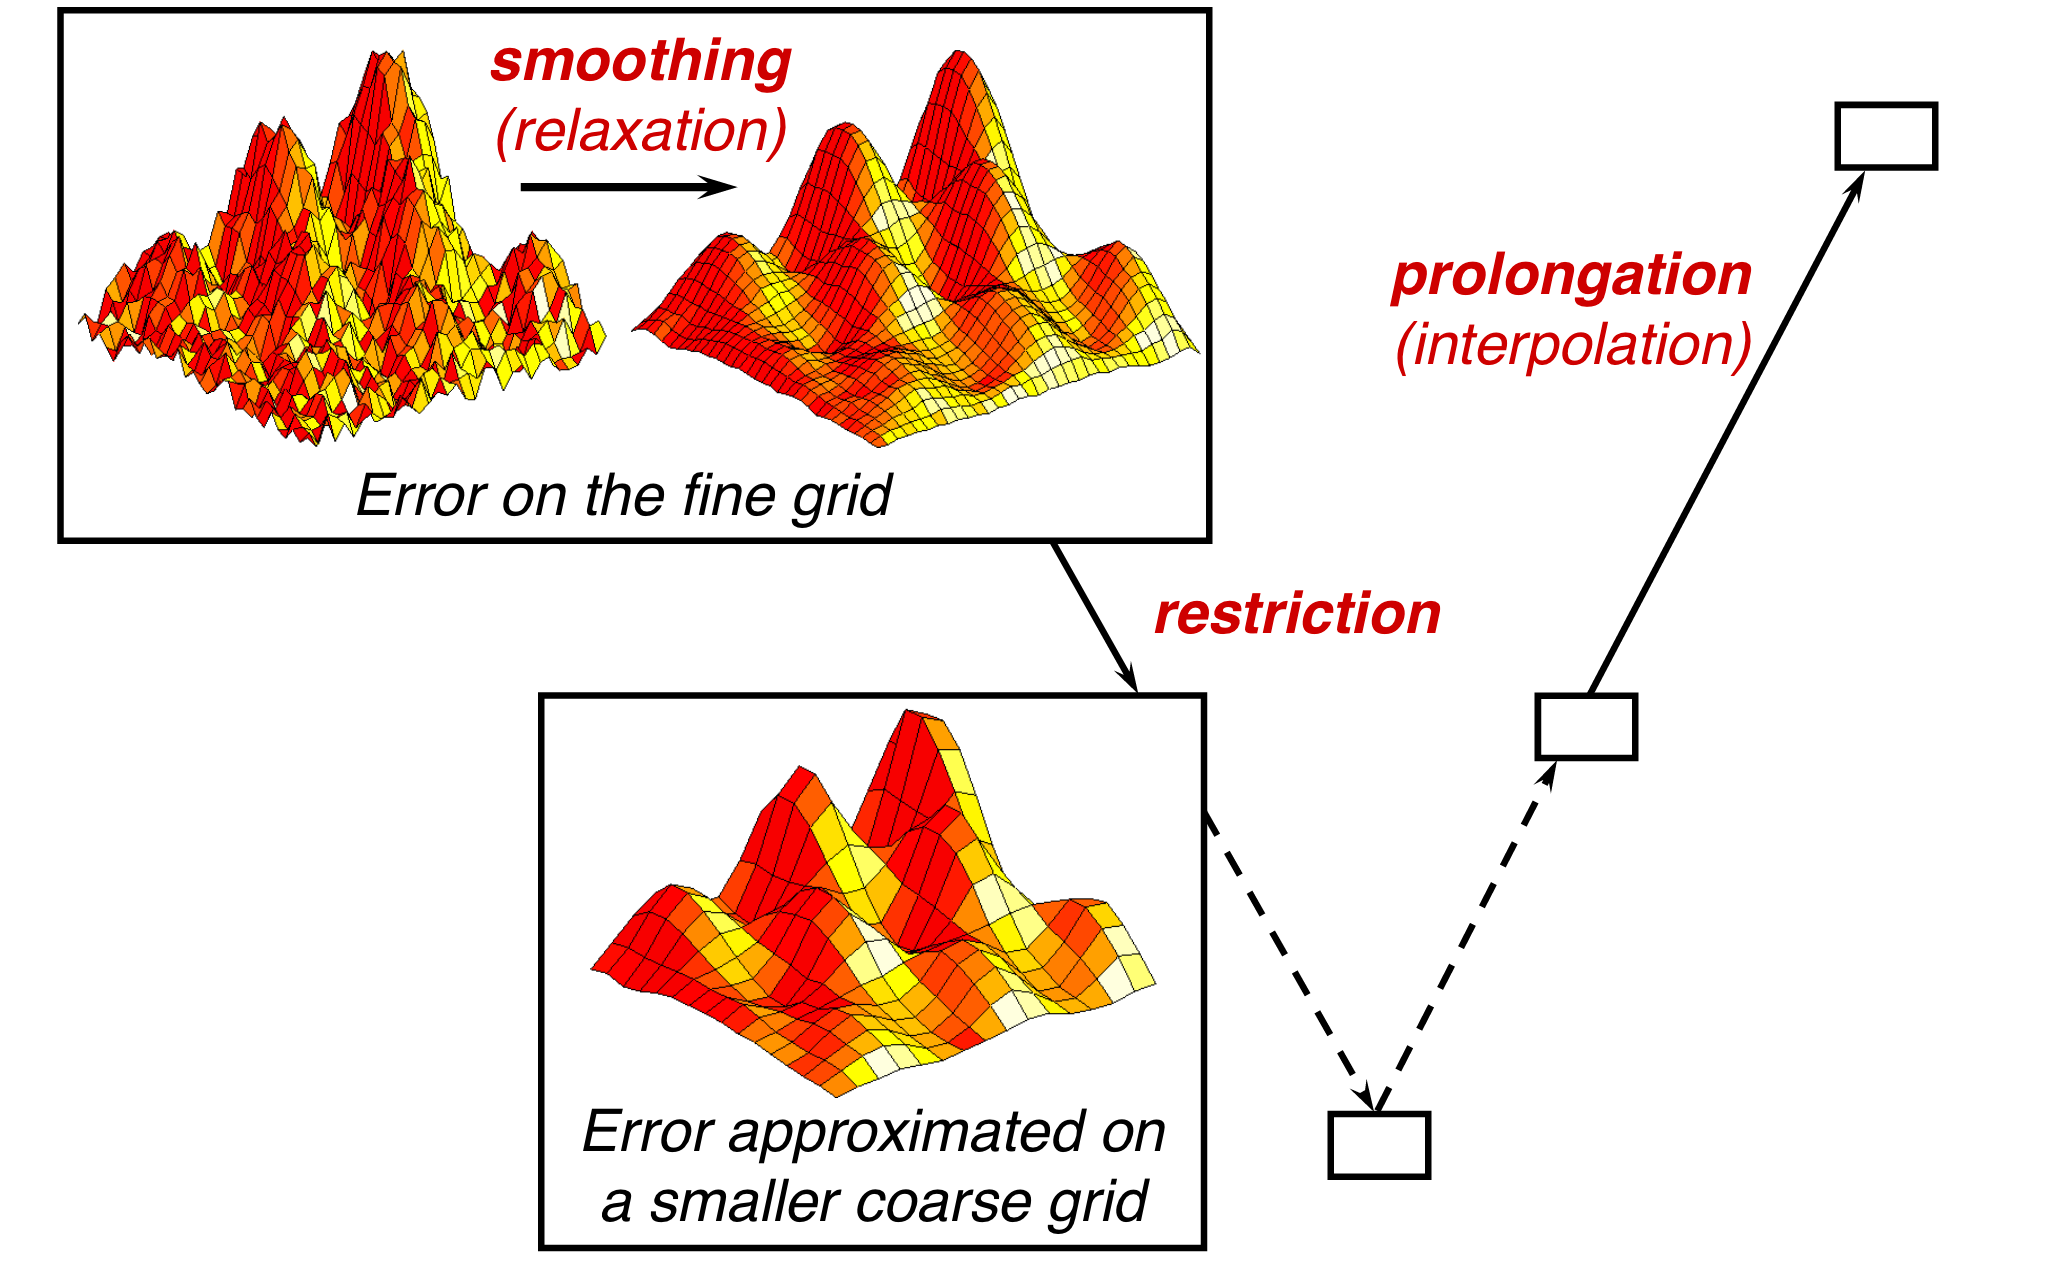
\includegraphics[width=1\textwidth]{Vcycle}
\end{frame}


\begin{frame}{Geometric multigrid (continued)}

\begin{description}[align=right]
  \item[Step 1:] smooth error (residual)
  \item[Step 2:] restrict to coarse grid
  \item[Step 3:] Solve on coarse grid
  \item[Step 4:] prolongate and correct
\end{description}

\end{frame}

\begin{frame}{Unstructured grids}
\begin{centering}

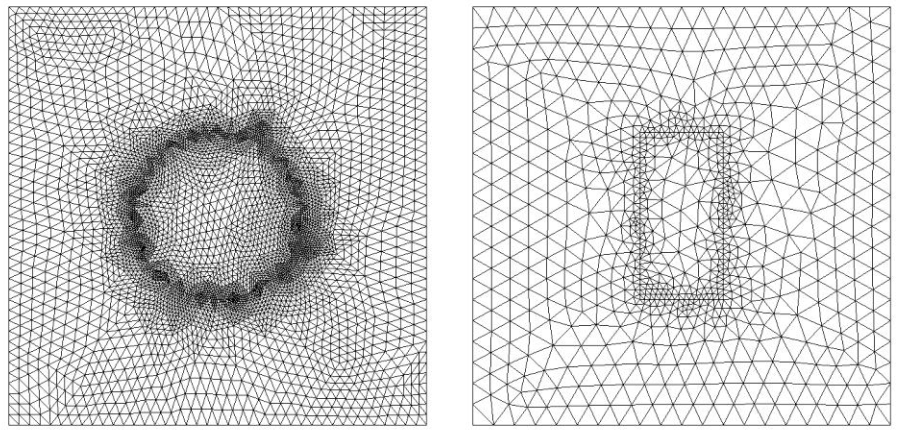
\includegraphics[width=.5\textwidth]{Grid1}\\

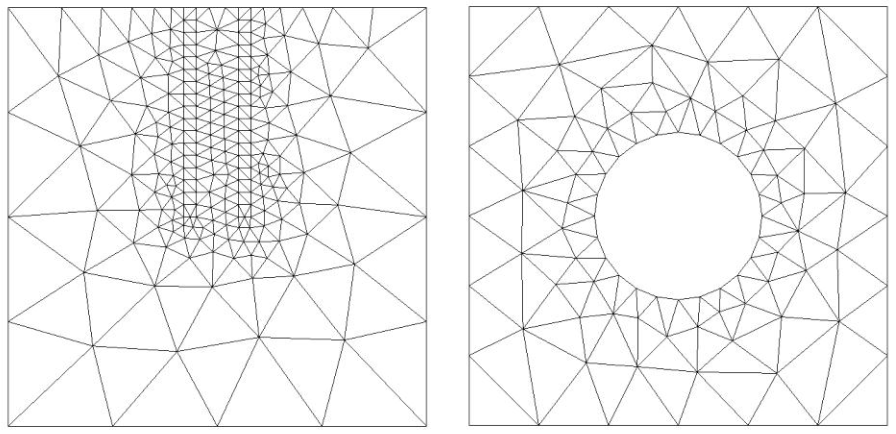
\includegraphics[width=.5\textwidth]{Grid2}

\end{centering}

\end{frame}

\section{AMG}
\begin{frame}{Algebraic Multigrid}
How do we do this in without defining a sequence of grids

\begin{itemize}
  \item Algebraic smoothness
  \item Algebraic restriction (how to define a sequence of grids)
\end{itemize}


\end{frame}





\begin{frame}

\textbf{Smoothness:}
$$e^{\mbox{\tiny{T}}}Ae = \lambda \ll 1$$


$$e^{\mbox{\tiny{T}}}Ae = \sum_{i<j} (-a_{ij})(e_i-e_j)^2 \ll 1$$


\textbf{Strength of Connection}
$$-a_{ij}\geq \theta \max_{k\neq i} \{-a_{ik}\} \ \ \ \mbox{where } \theta \in (0,1]$$


\end{frame}





\end{document}
